\documentclass[12pt,a4paper]{article}
\usepackage[latin1]{inputenc}
\usepackage[spanish]{babel}
\usepackage{amsmath}
\usepackage{amsfonts}
\usepackage{amssymb}
\usepackage{graphicx}
\usepackage[hidelinks]{hyperref}
\usepackage[left=2cm,right=2cm,top=2cm,bottom=2cm]{geometry}
\author{MEJORADA LOPEZ IVAN}
\title{GIRO DE UN MOTOR DE CORRIENTE DIRECTA}
\begin{document}
\maketitle

\includegraphics[width=18cm]{UPZMG_Prueba_1b.png}
\newpage
\section{MOTOR A CORRIENTE DIRECTA}
Los motores de Corriente Directa o motor DC(correspondiente a las iniciales en ingl\'es “direct current”) es tambi\'en conocidos como motor de Corriente Continua o motor CC, son  muy utilizados en dise\~nos de ingenier\'ia debido a las caracter\'isticas torque-velocidad que poseen con diferentes configuraciones el\'ectricas o mec\'anicas.\\Una gran ventaja de los motores de CD se debe a que es posible controlarlos con suavidad y en la mayor\'ia de los casos son reversibles, responden r\'apidamente gracias a que cuentan con una gran raz\'on de torque a la inercia del rotor.Otra ventaja es la implementaci\'on del frenado din\'amico, donde la energ\'ia generada por el motor se alimenta a un resistor disipador, y el frenado regenerativo donde la energ\'ia generada por el motor retroalimenta al suministro de potencia CD, esto es muy utilizado en aplicaciones donde se deseen frenados r\'apidos y de gran eficiencia.\\
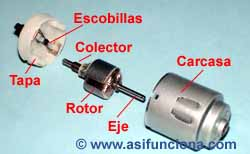
\includegraphics[width=15cm]{img14_mot_cd_250px.jpg} \\
El principio de funcionamiento de los motores el\'ectricos de corriente directa o continua se basa en la repulsi\'on que ejercen los polos magn\'eticos de un im\'an permanente cuando, de acuerdo con la Ley de Lorentz, interact\'uan con los polos magn\'eticos de un electroim\'an que se encuentra montado en un eje. Este electroim\'an se denomina “rotor” y su eje le permite girar libremente entre los polos magn\'eticos norte y sur del im\'an permanente situado dentro de la carcasa o cuerpo del motor.

Cuando la corriente el\'ectrica circula por la bobina de este electroim\'an giratorio, el campo electromagn\'etico que se genera interact\'ua con el campo magn\'etico del im\'an permanente. Si los polos del im\'an permanente y del electroim'an giratorio coinciden, se produce un rechazo y un torque magn\'etico o par de fuerza que provoca que el rotor rompa la inercia y comience a girar sobre su eje en el mismo sentido de las manecillas del reloj en unos casos, o en sentido contrario, de acuerdo con la forma que se encuentre conectada al circuito la pila o la bater\'ia.

\newpage
En todos los \'ambitos de la vida moderna podemos encontrar hoy en d\'ia muchos dispositivos \'a equipos que emplean motores el\'ectricos de diversos modelos, tama\~nos y potencias para realizar un determinado trabajo. Todos ellos, sin excepci\'on, funcionan con corriente alterna (C.A.), o de lo contrario con corriente directa (C.D.), conocida tambi\'en como corriente continua (C.C.). Sin embargo, la mayor\'ia de los dispositivos y equipos que requieren poca potencia para poner en funcionamiento sus mecanismos emplean solamente motores de corriente directa de peque\~no tama\~no, que utilizan como fuente suministradora de corriente el\'ectrica o fuerza electromotriz (F.E.M.) pilas, bater\'ia, o un convertidor de corriente alterna en directa.\\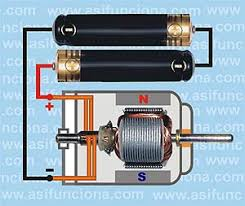
\includegraphics[width=11cm]{descarga.jpeg} \\
\section{Funci\'on del colector o conmutador en el motor de C.D.
}
En la siguiente figura se representa, de forma esquemática y simplificada, la vista frontal de un colector seccionado en dos partes, perteneciente a un motor de corriente directa (C.D.) muy simple. Tambi\'en se muestra el enrollado de la bobina del electroim\'an que gira a modo de rotor, diferenciada por un color diferente en cada una de sus mitades. Una de las mitades se representa por un c\'irculo rojo y la otra por un c\'irculo azul, identificados como 1 y 2. Como se puede ver, uno de los terminales de dicha bobina se encuentra conectado a la secci\'on “a” del colector y el otro terminal a la secci\'on b.
\newpage 
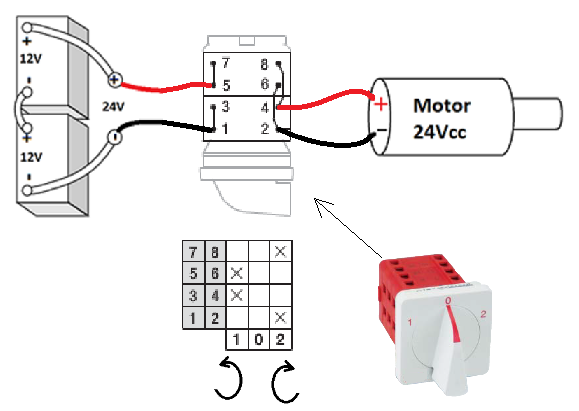
\includegraphics[scale=1]{conexion motor cc2.png} \\
La mayor\'ia de motores utilizados en la industria se conectan directamente a las l\'ineas de distribuci\'on el\'ectrica, y se alimentan con corriente alterna o corriente directa. Las terminales de los devanados del motor se conectan directamente a las l\'ineas de suministro el\'ectrico, y sus caracter\'isticas de operaci\'on se mantienen inalterables, al tener una tensi\'on de entrada constante. El motor trabaja en condiciones nominales cuando se alimenta con la tensi\'on indicada en la placa de operaci\'on, entregando potencia constante a la carga conectada en el eje.
\section{Forma de variar la velocidad de un motor DC en derivaci\'on}
*Ajustar el voltaje (y la corriente) aplicado al devanado del campo. Al aumentar el voltaje de campo, el motor desacelera.\\
*Ajustar el voltaje (y la corriente) aplicado a la armadura. Al aumentar el voltaje en la armadura el motor acelera.\\
\\
El control de armadura muchas veces se prefiere al de campo pues puede manejarse con más libertad la producci\'on de par con este m\'etodo.\\
\\
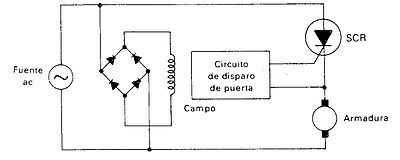
\includegraphics[width=15cm]{controlador_1.jpg}
\\
\section{BIBLIOGRAFIAS}
\url{http://www.asifunciona.com/electrotecnia/af_motor_cd/af_motor_cd_6.htm}
\\
\url{https://es.wikipedia.org/wiki/Control_de_motores_de_corriente_continua}
\\
\url{https://www.mecatronicalatam.com/motores/motores-de-cd}



\end{document}